\documentclass[]{elsarticle} %review=doublespace preprint=single 5p=2 column
%%% Begin My package additions %%%%%%%%%%%%%%%%%%%
\usepackage[hyphens]{url}

  \journal{Global Health Research and Policy - Thematic Series: Universal Health Coverage} % Sets Journal name


\usepackage{lineno} % add
\providecommand{\tightlist}{%
  \setlength{\itemsep}{0pt}\setlength{\parskip}{0pt}}

\bibliographystyle{elsarticle-harv}
\biboptions{sort&compress} % For natbib
\usepackage{graphicx}
\usepackage{booktabs} % book-quality tables
%%%%%%%%%%%%%%%% end my additions to header

\usepackage[T1]{fontenc}
\usepackage{lmodern}
\usepackage{amssymb,amsmath}
\usepackage{ifxetex,ifluatex}
\usepackage{fixltx2e} % provides \textsubscript
% use upquote if available, for straight quotes in verbatim environments
\IfFileExists{upquote.sty}{\usepackage{upquote}}{}
\ifnum 0\ifxetex 1\fi\ifluatex 1\fi=0 % if pdftex
  \usepackage[utf8]{inputenc}
\else % if luatex or xelatex
  \usepackage{fontspec}
  \ifxetex
    \usepackage{xltxtra,xunicode}
  \fi
  \defaultfontfeatures{Mapping=tex-text,Scale=MatchLowercase}
  \newcommand{\euro}{€}
\fi
% use microtype if available
\IfFileExists{microtype.sty}{\usepackage{microtype}}{}
\usepackage[left=3cm,right=3cm,top=3cm,bottom=3cm]{geometry}
\usepackage{longtable}
\usepackage{graphicx}
% We will generate all images so they have a width \maxwidth. This means
% that they will get their normal width if they fit onto the page, but
% are scaled down if they would overflow the margins.
\makeatletter
\def\maxwidth{\ifdim\Gin@nat@width>\linewidth\linewidth
\else\Gin@nat@width\fi}
\makeatother
\let\Oldincludegraphics\includegraphics
\renewcommand{\includegraphics}[1]{\Oldincludegraphics[width=\maxwidth]{#1}}
\ifxetex
  \usepackage[setpagesize=false, % page size defined by xetex
              unicode=false, % unicode breaks when used with xetex
              xetex]{hyperref}
\else
  \usepackage[unicode=true]{hyperref}
\fi
\hypersetup{breaklinks=true,
            bookmarks=true,
            pdfauthor={},
            pdftitle={Association between XXX and Life Expectency in 139 Countries: A Retrospective Longitudinal Study},
            colorlinks=true,
            urlcolor=blue,
            linkcolor=blue,
            pdfborder={0 0 0}}
\urlstyle{same}  % don't use monospace font for urls

\setcounter{secnumdepth}{5}
% Pandoc toggle for numbering sections (defaults to be off)
% Pandoc header
\usepackage{soulutf8}
\usepackage{color}
\usepackage{float}
\usepackage{booktabs}
\usepackage{lscape}
\usepackage{setspace}
\usepackage{dcolumn}



\begin{document}
\begin{frontmatter}

  \title{Association between XXX and Life Expectency in 139 Countries: A Retrospective Longitudinal Study}
    \author[SLU]{Miao Cai}
   \ead{miao.cai@slu.edu} 
  
    \author[SLU]{Asabe Garba}
   \ead{asabe.garba@slu.edu} 
  
    \author[WHU]{Xin Li}
   \ead{xl60@iu.edu} 
  
    \author[SCU]{Xiaojun Lin\corref{c1}}
   \ead{xjlin@hust.edu.cn} 
   \cortext[c1]{Corresponding Author}
      \address[SLU]{Saint Louis University, Saint Louis, MO, 63108}
    \address[SCU]{Sichuan University, Chengdu, Sichuan, China}
    \address[WHU]{Wuhan University, Wuhan, Hubei, China}
  
  \begin{abstract}
  This is the abstract.
  
  It consists of two paragraphs.
  \end{abstract}
  
 \end{frontmatter}

\newcommand{\blandscape}{\begin{landscape}}
\newcommand{\elandscape}{\end{landscape}}
\doublespacing

\hypertarget{introduction}{%
\section{Introduction}\label{introduction}}

\hl{government health expenditure and life expectancy.}

{[}\protect\hyperlink{ref-wagstaff2018progress}{1}{]}.

\hypertarget{special-issue-information}{%
\section{Special issue information}\label{special-issue-information}}

Universal health coverage (UHC) is one of the key approaches in achieving the 2030 Agenda for Sustainable Development Goals (SDGs). On October 25-26, 2018, the Global Conference on Primary Health Care was held in Kazakhstan, and the Declaration of Astana was signed by 197 Member States under the leadership of the World Health Organization (WHO). In this Declaration, strengthening primary health care system has been considered as an essential step towards achieving Universal Health Coverage.

This thematic series of articles is being launched by the Global Health Research and Policy (GHRP) to serve as a platform to disseminate current research findings, insights, new perspectives, and policy recommendations in promoting UHC worldwide. This will serve to create better knowledge transfer from researches to policy-making and practices and for information and experience sharing. GHRP is encouraging submissions of commentaries, reviews, research articles, and short report of policies on the key elements of UHC. Elements that can be covered in the submissions may include, but not limited to the following:

\begin{itemize}
\item
  Health financing system strengthening, with special focus on the development of health financial protection schemes for the disadvantaged population, as well as the integration of different insurance programs.
\item
  Primary healthcare system strengthening, with special focus on health workforce and delivery network of primary health care services, equity and quality of primary health care, information systems construction, etc.
\item
  People-centered health care system, with special focus on the integration of specialist healthcare services and primary health care, and the provision of continuous services to improve patient experience, etc.
\item
  Essential medicines and health products, with special focus on strategic purchasing, relevant mechanism designs and market entry for insurance benefit package.
\item
  Medical assistance programs for poverty alleviation as an approach to increase UHC.
\end{itemize}

This thematic series will be guest edited by Dr.~Beibei Yuan (beibeiyuan@bjmu.edu.cn), Associate Professor from Peking University and Dr.~Lanting Lu (lanting.lu@ruc.edu.cn), Associate Professor from Renmin University of China.

Submissions from anywhere in the world are welcome. Authors are advised to select the Thematic Series option ``Universal Health Coverage'' during their submission. The deadline of submission is on \textbf{April 14, 2019}.

\hypertarget{methods}{%
\section{Methods}\label{methods}}

\hypertarget{data-souce}{%
\subsection{Data souce}\label{data-souce}}

We extracted country level data from the Global Health Expenditure Database on the World Health Organization (WHO) website.{[}\protect\hyperlink{ref-WHOdata}{2}{]} This database includes comparable health expenditure data for around 190 countries from 2000 to 2016. Besides, we downloaded Life expectancy data by country from the Global Health Observatory data repository provided by the WHO.{[}\protect\hyperlink{ref-WHOlife}{3}{]}

\hypertarget{variable-selection}{%
\subsection{Variable selection}\label{variable-selection}}

Outcome: life expectancy

Independent variables: life expectancy

Variable selection:

\begin{itemize}
\tightlist
\item
  Current Health Expenditure (CHE) as \% GDP: CHEGDP\_SHA2011
\item
  Government Health Expenditure (GGHE-D) as \% GDP: GGHEDGDP\_SHA2011
\item
  Domestic Private Health Expenditure (PVT-D) as \% CHE: PVTDCHE\_SHA2011
\item
  Compulsory Financing Arrangements (CFA) as \% of CHE: CFACHE\_SHA2011
\item
  OOP \% CHE: OOPSCHE\_SHA2011
\item
  Population
\item
  GDP
\item
  Year
\end{itemize}

Multi-collinearity:

CFACHE\_SHA2011 - kept only
GFACHE\_SHA2011
CHICHE\_SHA2011

\hypertarget{statistical-analyses}{%
\subsection{Statistical Analyses}\label{statistical-analyses}}

Point and interval estimates (95\% confidence intervals, 95\% CI), as well as the p-values, were reported for all indepdent variables. A p-value less than 0.05 is viewed as statistically significant. All data cleaning, visualization, statistical modelling, and reporting were performed using R 3.5.3 {[}\protect\hyperlink{ref-R353}{4}{]}. In an effort to promote reproducible research, we have created a public GitHub repository to store all the data and R code we use to write this paper.
Interested readers can find them at \url{https://github.com/caimiao0714/GHRP-UHC}.

\hypertarget{results}{%
\section{Results}\label{results}}

\begin{figure}
\centering
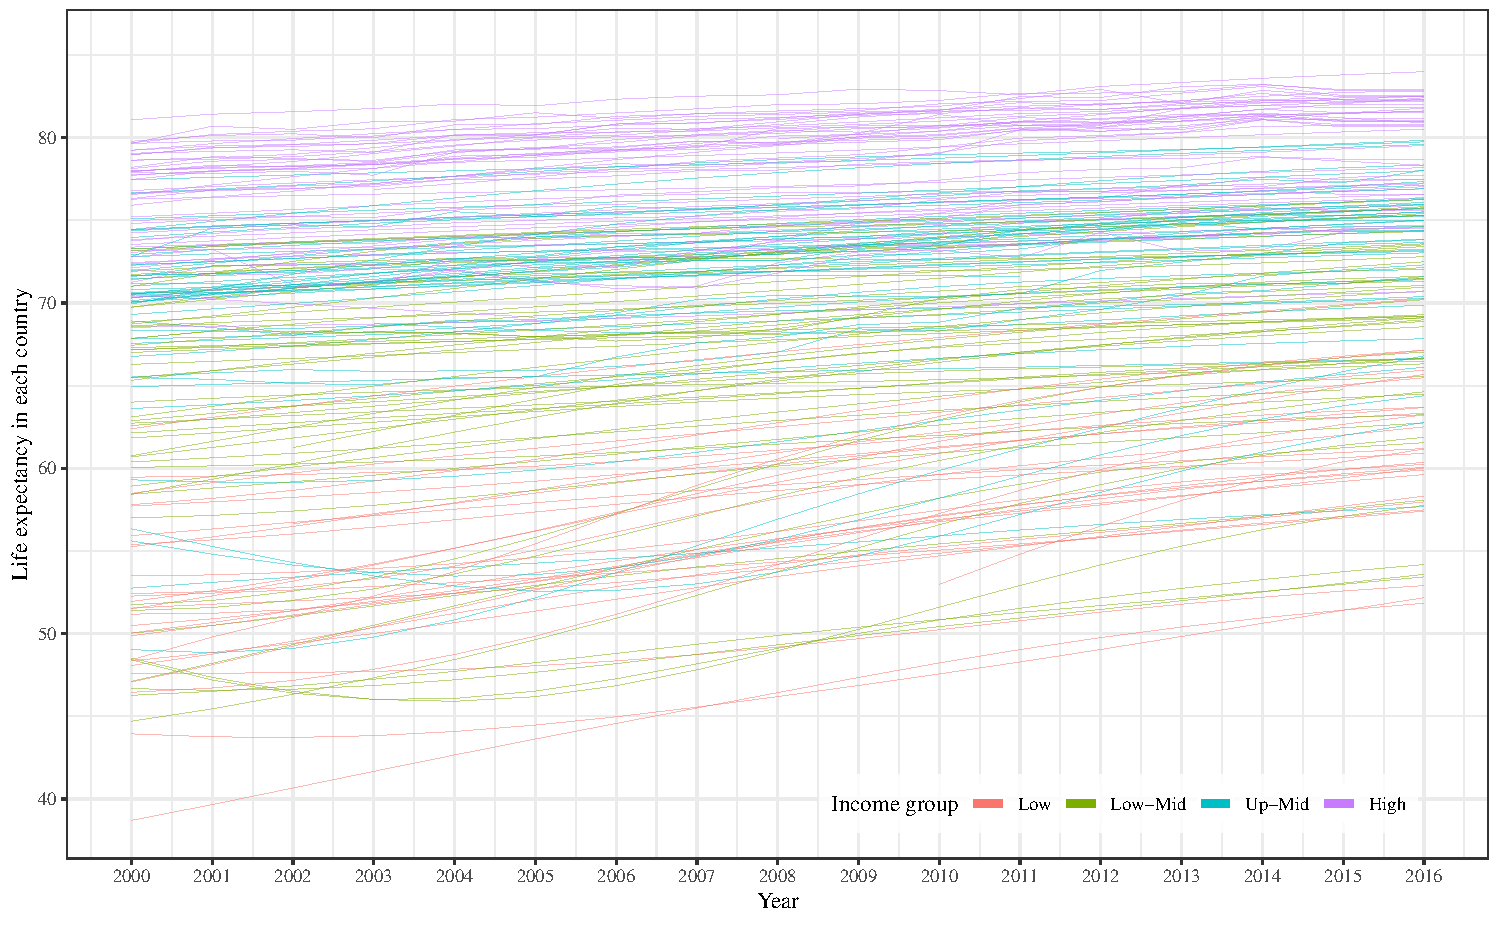
\includegraphics{Figures/fig1.pdf}
\caption{\label{fig:fig1}Life expectancy in 139 countries from 2000 to 2015}
\end{figure}

Figure \ref{fig:fig1}

\hl{Xiaojun Lin, create the Table 1 for f1. write results for Table 1, 2, 3 and Figure 1.}

\begin{table}[!htbp] \centering 
  \caption{OLS model predicting life expectancies in 139 countries from 2000 to 2015} 
  \label{poolOLS} 
\begin{tabular}{@{\extracolsep{5pt}}lc} 
\\[-1.8ex]\hline 
\hline \\[-1.8ex] 
 & \multicolumn{1}{c}{\textit{Dependent variable:}} \\ 
\cline{2-2} 
\\[-1.8ex] & Life expectancy \\ 
\hline \\[-1.8ex] 
 Current Health Expenditure as percent of GDP & 0.067 \\ 
  & ($-$0.120, 0.253) \\ 
  & \\ 
 Government Health Expenditure as percent of GDP & 1.065$^{***}$ \\ 
  & (0.744, 1.385) \\ 
  & \\ 
 Private Health Expenditure as percent CHE & $-$0.146$^{***}$ \\ 
  & ($-$0.186, $-$0.105) \\ 
  & \\ 
 Compulsory Financing Arrangements as percent of CHE & $-$0.001 \\ 
  & ($-$0.022, 0.019) \\ 
  & \\ 
 Out-of-pocket payment as percent of CHE & 0.200$^{***}$ \\ 
  & (0.165, 0.236) \\ 
  & \\ 
 Population (millions) & 0.002 \\ 
  & ($-$0.002, 0.006) \\ 
  & \\ 
 GDP & 0.035$^{***}$ \\ 
  & (0.013, 0.057) \\ 
  & \\ 
 Year & 0.335$^{***}$ \\ 
  & (0.282, 0.387) \\ 
  & \\ 
 Low income country & $-$18.672$^{***}$ \\ 
  & ($-$19.837, $-$17.508) \\ 
  & \\ 
 Low to middle income country & $-$11.030$^{***}$ \\ 
  & ($-$11.951, $-$10.109) \\ 
  & \\ 
 Up to middel income country & $-$5.152$^{***}$ \\ 
  & ($-$5.985, $-$4.319) \\ 
  & \\ 
 Constant & $-$600.036$^{***}$ \\ 
  & ($-$705.527, $-$494.546) \\ 
  & \\ 
\hline \\[-1.8ex] 
Observations & 2,189 \\ 
R$^{2}$ & 0.675 \\ 
Adjusted R$^{2}$ & 0.673 \\ 
\hline 
\hline \\[-1.8ex] 
\textit{Note:}  & \multicolumn{1}{l}{$^{*}$p$<$0.1; $^{**}$p$<$0.05; $^{***}$p$<$0.01} \\ 
 & \multicolumn{1}{l}{CHE: Current Health Expenditure,} \\ 
 & \multicolumn{1}{l}{GDP: Gross Domestic Product} \\ 
 & \multicolumn{1}{l}{GHE: Government Health Expenditure} \\ 
 & \multicolumn{1}{l}{PVT-D: Private Health Expenditure} \\ 
 & \multicolumn{1}{l}{OOP: Out-of-pocket payment} \\ 
 & \multicolumn{1}{l}{CFA: Compulsory Financing Arrangements} \\ 
\end{tabular} 
\end{table}

Table \ref{poolOLS} demonstrates XXXXXXX.

\begin{landscape}

\begin{table}[!htbp] \centering 
  \caption{OLS model predicting life expectancies from 2000 to 2015 stratifeid by country income categories} 
  \label{stratifiedOLS} 
\begin{tabular}{@{\extracolsep{5pt}}lD{.}{.}{-3} D{.}{.}{-3} D{.}{.}{-3} D{.}{.}{-3} } 
\\[-1.8ex]\hline 
\hline \\[-1.8ex] 
 & \multicolumn{4}{c}{\textit{Dependent variable:}} \\ 
\cline{2-5} 
\\[-1.8ex] & \multicolumn{4}{c}{Life expectancy} \\ 
 & \multicolumn{1}{c}{Low} & \multicolumn{1}{c}{Low-mid} & \multicolumn{1}{c}{Up-mid} & \multicolumn{1}{c}{High} \\ 
\\[-1.8ex] & \multicolumn{1}{c}{(1)} & \multicolumn{1}{c}{(2)} & \multicolumn{1}{c}{(3)} & \multicolumn{1}{c}{(4)}\\ 
\hline \\[-1.8ex] 
 Current Health Expenditure as percent of GDP & -0.532^{***} & 0.790^{***} & 0.943^{***} & 1.062^{**} \\ 
  & \multicolumn{1}{c}{(-0.801$, $-0.262)} & \multicolumn{1}{c}{(0.286$, $1.294)} & \multicolumn{1}{c}{(0.380$, $1.506)} & \multicolumn{1}{c}{(0.211$, $1.913)} \\ 
  & & & & \\ 
 Government Health Expenditure as percent of GDP & 0.378 & -0.547 & -0.224 & 0.274 \\ 
  & \multicolumn{1}{c}{(-0.617$, $1.372)} & \multicolumn{1}{c}{(-1.432$, $0.338)} & \multicolumn{1}{c}{(-1.225$, $0.777)} & \multicolumn{1}{c}{(-0.815$, $1.363)} \\ 
  & & & & \\ 
 Private Health Expenditure as percent CHE & 0.207^{***} & -0.320^{***} & -0.206^{***} & -0.050 \\ 
  & \multicolumn{1}{c}{(0.094$, $0.320)} & \multicolumn{1}{c}{(-0.437$, $-0.202)} & \multicolumn{1}{c}{(-0.298$, $-0.113)} & \multicolumn{1}{c}{(-0.155$, $0.054)} \\ 
  & & & & \\ 
 Compulsory Financing Arrangements as percent of CHE & -0.069^{**} & 0.125^{***} & 0.118^{***} & -0.001 \\ 
  & \multicolumn{1}{c}{(-0.134$, $-0.004)} & \multicolumn{1}{c}{(0.036$, $0.214)} & \multicolumn{1}{c}{(0.049$, $0.188)} & \multicolumn{1}{c}{(-0.015$, $0.013)} \\ 
  & & & & \\ 
 Out-of-pocket payment as percent of CHE & -0.187^{***} & 0.445^{***} & 0.279^{***} & 0.044 \\ 
  & \multicolumn{1}{c}{(-0.293$, $-0.082)} & \multicolumn{1}{c}{(0.334$, $0.555)} & \multicolumn{1}{c}{(0.233$, $0.326)} & \multicolumn{1}{c}{(-0.013$, $0.102)} \\ 
  & & & & \\ 
 Population (millions) & 0.040^{**} & 0.001 & 0.020^{***} & -0.003 \\ 
  & \multicolumn{1}{c}{(0.002$, $0.078)} & \multicolumn{1}{c}{(-0.004$, $0.007)} & \multicolumn{1}{c}{(0.005$, $0.034)} & \multicolumn{1}{c}{(-0.021$, $0.014)} \\ 
  & & & & \\ 
 GDP & 0.121 & 1.454^{***} & -0.095 & 0.029^{***} \\ 
  & \multicolumn{1}{c}{(-2.150$, $2.393)} & \multicolumn{1}{c}{(0.895$, $2.013)} & \multicolumn{1}{c}{(-0.215$, $0.026)} & \multicolumn{1}{c}{(0.016$, $0.042)} \\ 
  & & & & \\ 
 Year & 0.650^{***} & 0.182^{***} & 0.252^{***} & 0.150^{***} \\ 
  & \multicolumn{1}{c}{(0.523$, $0.777)} & \multicolumn{1}{c}{(0.047$, $0.317)} & \multicolumn{1}{c}{(0.160$, $0.345)} & \multicolumn{1}{c}{(0.088$, $0.212)} \\ 
  & & & & \\ 
 Constant & -1,245.363^{***} & -314.655^{**} & -447.064^{***} & -231.842^{***} \\ 
  & \multicolumn{1}{c}{(-1,500.030$, $-990.696)} & \multicolumn{1}{c}{(-586.047$, $-43.263)} & \multicolumn{1}{c}{(-632.238$, $-261.889)} & \multicolumn{1}{c}{(-355.918$, $-107.765)} \\ 
  & & & & \\ 
\hline \\[-1.8ex] 
Observations & \multicolumn{1}{c}{384} & \multicolumn{1}{c}{620} & \multicolumn{1}{c}{652} & \multicolumn{1}{c}{533} \\ 
R$^{2}$ & \multicolumn{1}{c}{0.315} & \multicolumn{1}{c}{0.203} & \multicolumn{1}{c}{0.307} & \multicolumn{1}{c}{0.478} \\ 
Adjusted R$^{2}$ & \multicolumn{1}{c}{0.300} & \multicolumn{1}{c}{0.192} & \multicolumn{1}{c}{0.298} & \multicolumn{1}{c}{0.470} \\ 
\hline 
\hline \\[-1.8ex] 
\textit{Note:}  & \multicolumn{4}{r}{$^{*}$p$<$0.1; $^{**}$p$<$0.05; $^{***}$p$<$0.01} \\ 
\end{tabular} 
\end{table} 
\end{landscape}

Table \ref{stratifiedOLS} presents XXXXXXX.

\hypertarget{discussion}{%
\section{Discussion}\label{discussion}}

\hypertarget{references}{%
\section*{References}\label{references}}
\addcontentsline{toc}{section}{References}

\hypertarget{refs}{}
\leavevmode\hypertarget{ref-wagstaff2018progress}{}%
1. Wagstaff A, Flores G, Smitz M-F, Hsu J, Chepynoga K, Eozenou P. Progress on impoverishing health spending in 122 countries: A retrospective observational study. The Lancet Global Health. 2018;6:e180--92.

\leavevmode\hypertarget{ref-WHOdata}{}%
2. The World Health Organization. Global Health Expenditure Database. 2016. \url{http://apps.who.int/nha/database/Select/Indicators/en}. Accessed 20 Mar 2019.

\leavevmode\hypertarget{ref-WHOlife}{}%
3. The World Health Organization. Global Health Observatory data repository. 2018. \url{http://apps.who.int/nha/database/Select/Indicators/en}. Accessed 6 Apr 2018.

\leavevmode\hypertarget{ref-R353}{}%
4. R Core Team. R: A language and environment for statistical computing. Vienna, Austria: R Foundation for Statistical Computing; 2019. \url{https://www.R-project.org/}.

\end{document}


